% Capa
\imprimircapa

% Folha de rosto
\imprimirfolhaderosto*

\begin{fichacatalografica}
	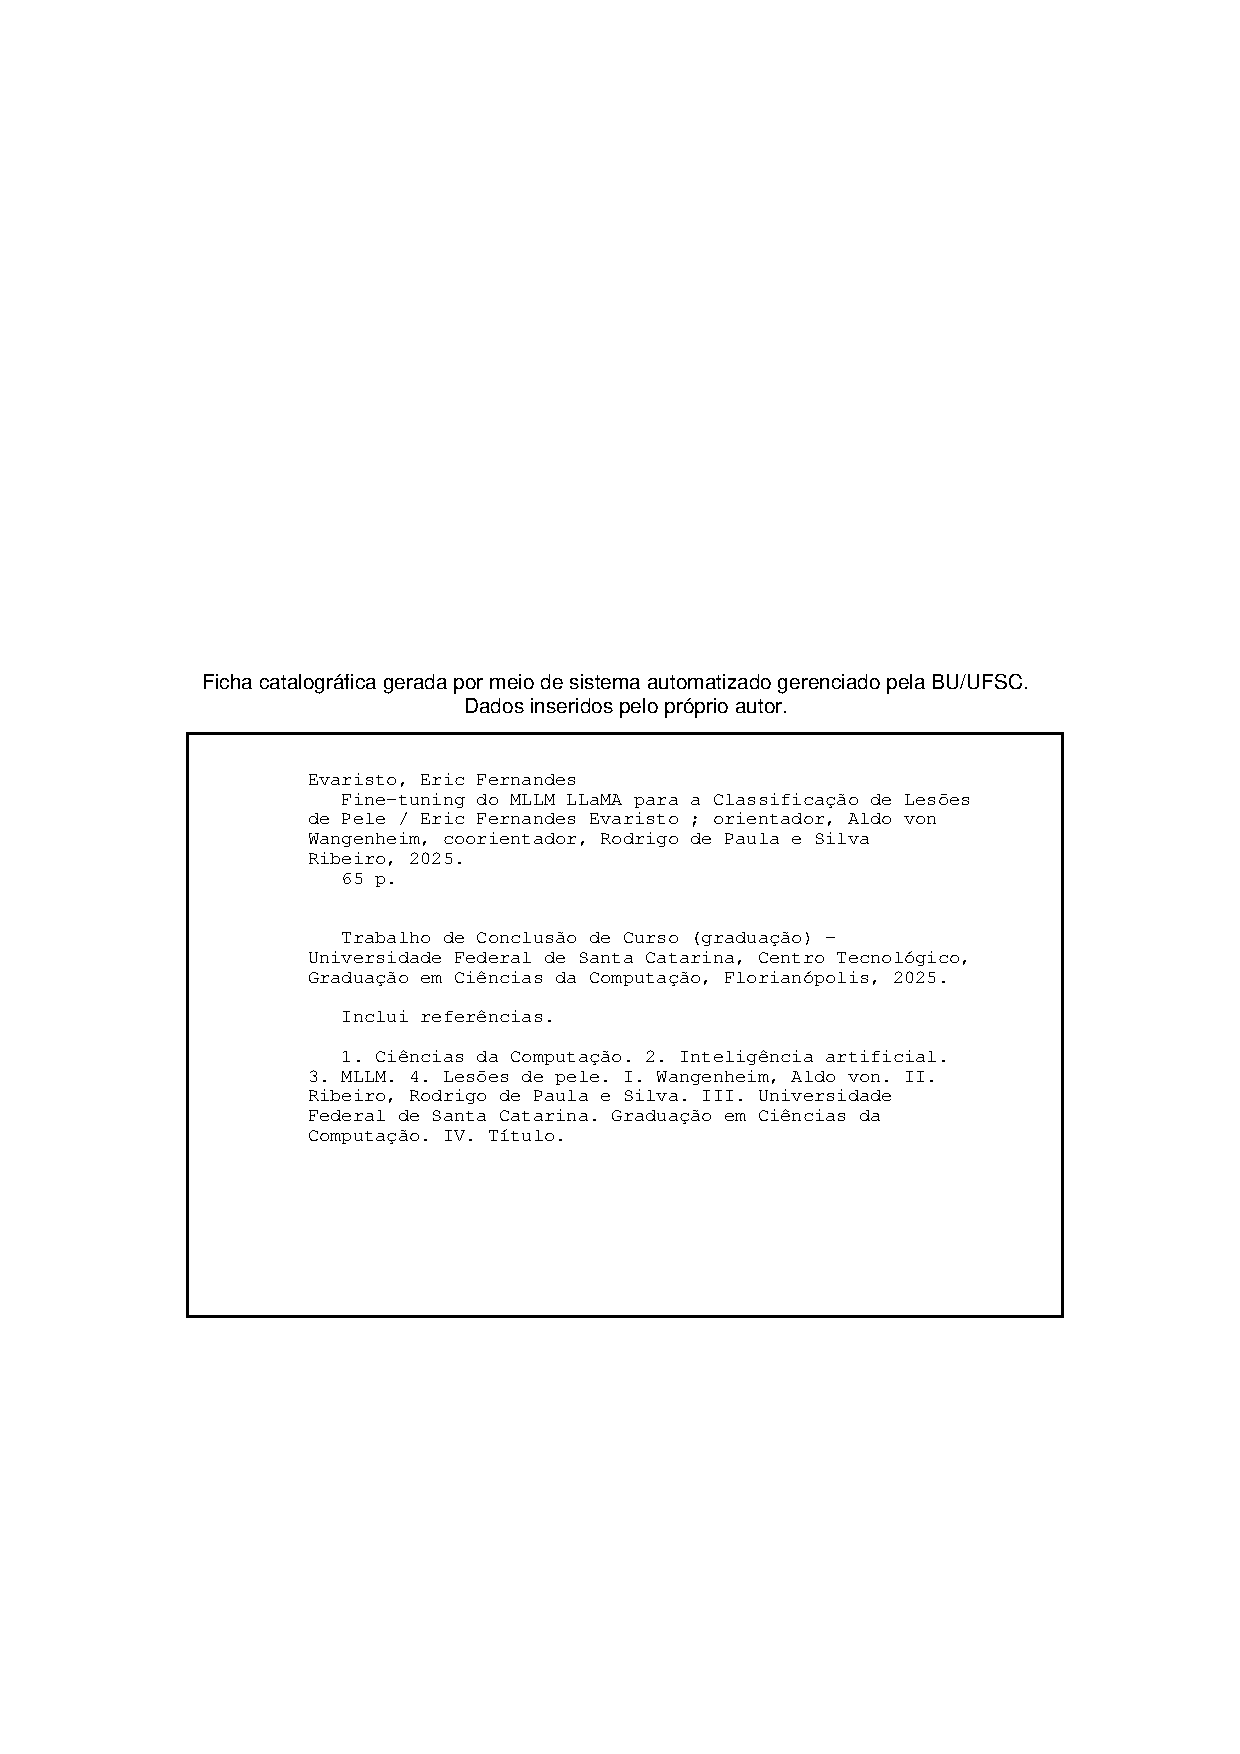
\includepdf{beforetext/Ficha_Catalografica.pdf}
\end{fichacatalografica}

% Folha de aprovação
\begin{folhadeaprovacao}
	\begin{center}
		{\imprimirautor}

		\begin{center}
			\ABNTEXchapterfont\bfseries\MakeUppercase{\imprimirtitulo}\ifnotempty{\imprimirsubtitulo}{: \imprimirsubtitulo}
		\end{center}

		\begin{minipage}{\textwidth}
			Este Trabalho de Conclusão de Curso foi julgado adequado para obtenção do Título de \imprimirformacao,
			e foi aprovado em sua forma final pelo Curso de Ciência da Computação.
		\end{minipage}%
	\end{center}

	\begin{center}
		\imprimirlocal, 15 de julho de 2025.
	\end{center}

	\assinatura{
		\textbf{\imprimircoordenador} \\
		Coordenação do Curso
	}

	\begin{center}
		\vspace{1cm}
		\textbf{Banca Examinadora:}
	\end{center}

	\vspace{1cm}
	\assinatura{
		\textbf{\imprimirorientador} \\ \imprimirorientadorRotulo
	}

	% \imprimircoorientador{
	% 	\assinatura{
	% 		\textbf{\imprimircoorientador} \\ \imprimircoorientadorRotulo \\
	% 		\imprimirinstituicao~--~\imprimirinstituicaosigla
	% 	}
	% }

	\vspace{1cm}
	\assinatura{
		\textbf{Prof. Convidado 1, Dr.} \\
		Instituição 1 -- Sigla 1
	}

	\vspace{1cm}
	\assinatura{
		\textbf{Prof. Convidado 2, Dr.} \\
		Instituição 2 -- Sigla 2
	}

	\begin{center}
		\vfill
		{
			\imprimirlocal\par
			\imprimirano\par
		}
	\end{center}
\end{folhadeaprovacao}

% \begin{agradecimentos}
    ...
\end{agradecimentos}

% Resumo em português
\setlength{\absparsep}{18pt}
\begin{resumo}
	\SingleSpacing
	Lesões de pele podem ser um indicativo de diversas doenças, incluindo doenças graves como o câncer de pele. A detecção precoce dessas lesões é fundamental para o
	tratamento e cura da doença. Porém, o diagnóstico e classificação de uma lesão de pele é normalmente feita por profissionais especializados em hospitais ou clínicas.
	Isto pode levar a um atraso no diagnóstico pela falta de acesso ou procura pelo atendimento médico.

	Considerando este cenário, tecnologias como \acp{MLLM} podem ser úteis. Estes modelos podem identificar e classificar lesões de pele com base em imagens e prover um
	pré-diagnóstico compreensível ao portador da lesão, indicando a necessidade de procurar atendimento médico. O modelo \ac{LLaMA 3.2} é um bom candidato para esta
	aplicação, pois consegue descrever imagens e pode ser adaptado para propósitos específicos através de \textit{fine-tuning}.

	Neste trabalho, propõe-se a adaptação do \ac{LLaMA 3.2} com diferentes técnicas de \textit{fine-tuning} baseadas em \ac{PEFT}, comparando-as entre si, para
	classificar lesões de pele com uma precisão aceitável. Por conta da severidade, será dado um foco maior à detecção de câncer de pele.

	\textbf{Palavras-chave}: Lesões de pele. Câncer de pele. MLLM. LLaMA. PEFT. Fine tuning.
\end{resumo}

% Resumo em inglês
\begin{resumo}[Abstract]
	\SingleSpacing
	\begin{otherlanguage*}{english}
		Skin lesions can indicate several diseases, including serious diseases such as skin cancer. Early detection of these lesions is essential for the treatment
		and cure of the disease. However, the diagnosis and classification of a skin lesion is normally carried out by specialized professionals in hospitals or clinics.
		This can lead to a delay in diagnosis due to a lack of access to or demand for medical care.

		Considering this scenario, technologies like \acp{MLLM} can be useful. These models can identify and classify skin lesions based on images and provide an
		understandable pre-diagnosis to the affected person, indicating the need to seek medical attention. The \ac{LLaMA 3.2} model  is a good candidate for this
		application, as it can describe images and be adapted for specific purposes through fine-tuning.

		In this work, we propose the adaptation of \ac{LLaMA 3.2} with different fine-tuning techniques, comparing them to each other, to classify skin lesions with an
		acceptable accuracy. Because of its severity, there will be a greater focus on detecting skin cancer.

		\textbf{Keywords}: Skin lesions. Skin cancer. MLLM. LLaMA. PEFT. Fine tuning.
	\end{otherlanguage*}
\end{resumo}

{
\hypersetup{hidelinks}

% Lista de imagens
\pdfbookmark[0]{\listfigurename}{lof}
\listoffigures

% Lista de siglas
\imprimirlistadesiglas

% Sumário
\pdfbookmark[0]{\contentsname}{toc}
\tableofcontents*
\cleardoublepage
}
